%**************************************%
%* Generated from MathBook XML source *%
%*    on 2016-08-14T13:17:45-04:00    *%
%*                                    *%
%*   http://mathbook.pugetsound.edu   *%
%*                                    *%
%**************************************%
\documentclass[10pt,]{book}
%% Load geometry package to allow page margin adjustments
\usepackage{geometry}
\geometry{letterpaper,total={5.0in,9.0in}}
%% Custom Preamble Entries, early (use latex.preamble.early)
%% Inline math delimiters, \(, \), need to be robust
%% 2016-01-31:  latexrelease.sty  supersedes  fixltx2e.sty
%% If  latexrelease.sty  exists, bugfix is in kernel
%% If not, bugfix is in  fixltx2e.sty
%% See:  https://tug.org/TUGboat/tb36-3/tb114ltnews22.pdf
%% and read "Fewer fragile commands" in distribution's  latexchanges.pdf
\IfFileExists{latexrelease.sty}{}{\usepackage{fixltx2e}}
%% Page Layout Adjustments (latex.geometry)
%% This LaTeX file may be compiled with pdflatex, xelatex, or lualatex
%% The following provides engine-specific capabilities
%% Generally, xelatex and lualatex will do better languages other than US English
%% You can pick from the conditional if you will only ever use one engine
\usepackage{ifthen}
\usepackage{ifxetex,ifluatex}
\ifthenelse{\boolean{xetex} \or \boolean{luatex}}{%
%% begin: xelatex and lualatex-specific configuration
%% fontspec package will make Latin Modern (lmodern) the default font
\ifxetex\usepackage{xltxtra}\fi
\usepackage{fontspec}
%% realscripts is the only part of xltxtra relevant to lualatex 
\ifluatex\usepackage{realscripts}\fi
%% 
%% Extensive support for other languages
\usepackage{polyglossia}
\setdefaultlanguage{english}
%% Magyar (Hungarian)
\setotherlanguage{magyar}
%% Spanish
\setotherlanguage{spanish}
%% Vietnamese
\setotherlanguage{vietnamese}
%% end: xelatex and lualatex-specific configuration
}{%
%% begin: pdflatex-specific configuration
%% translate common Unicode to their LaTeX equivalents
%% Also, fontenc with T1 makes CM-Super the default font
%% (\input{ix-utf8enc.dfu} from the "inputenx" package is possible addition (broken?)
\usepackage[T1]{fontenc}
\usepackage[utf8]{inputenc}
%% end: pdflatex-specific configuration
}
%% Monospace font: Inconsolata (zi4)
%% Sponsored by TUG: http://levien.com/type/myfonts/inconsolata.html
%% See package documentation for excellent instructions
%% One caveat, seem to need full file name to locate OTF files
%% Loads the "upquote" package as needed, so we don't have to
%% Upright quotes might come from the  textcomp  package, which we also use
%% We employ the shapely \ell to match Google Font version
%% pdflatex: "varqu" option produces best upright quotes
%% xelatex,lualatex: add StylisticSet 1 for shapely \ell
%% xelatex,lualatex: add StylisticSet 2 for plain zero
%% xelatex,lualatex: we add StylisticSet 3 for upright quotes
%% 
\ifthenelse{\boolean{xetex} \or \boolean{luatex}}{%
%% begin: xelatex and lualatex-specific monospace font
\usepackage{zi4}
\setmonofont[BoldFont=Inconsolatazi4-Bold.otf,StylisticSet={1,3}]{Inconsolatazi4-Regular.otf}
%% end: xelatex and lualatex-specific monospace font
}{%
%% begin: pdflatex-specific monospace font
\usepackage[varqu]{zi4}
%% end: pdflatex-specific monospace font
}
%% Symbols, align environment, bracket-matrix
\usepackage{amsmath}
\usepackage{amssymb}
%% allow more columns to a matrix
%% can make this even bigger by overriding with  latex.preamble.late  processing option
\setcounter{MaxMatrixCols}{30}
%%
%% Color support, xcolor package
%% Always loaded.  Used for:
%% mdframed boxes, add/delete text, author tools
\PassOptionsToPackage{usenames,dvipsnames,svgnames,table}{xcolor}
\usepackage{xcolor}
%%
%% Semantic Macros
%% To preserve meaning in a LaTeX file
%% Only defined here if required in this document
%% Subdivision Numbering, Chapters, Sections, Subsections, etc
%% Subdivision numbers may be turned off at some level ("depth")
%% A section *always* has depth 1, contrary to us counting from the document root
%% The latex default is 3.  If a larger number is present here, then
%% removing this command may make some cross-references ambiguous
%% The precursor variable $numbering-maxlevel is checked for consistency in the common XSL file
\setcounter{secnumdepth}{3}
%% Environments with amsthm package
%% Theorem-like environments in "plain" style, with or without proof
\usepackage{amsthm}
\theoremstyle{plain}
%% Numbering for Theorems, Conjectures, Examples, Figures, etc
%% Controlled by  numbering.theorems.level  processing parameter
%% Always need a theorem environment to set base numbering scheme
%% even if document has no theorems (but has other environments)
\newtheorem{theorem}{Theorem}[section]
%% Only variants actually used in document appear here
%% Style is like a theorem, and for statements without proofs
%% Numbering: all theorem-like numbered consecutively
%% i.e. Corollary 4.3 follows Theorem 4.2
%% Definition-like environments, normal text
%% Numbering is in sync with theorems, etc
\theoremstyle{definition}
\newtheorem{definition}[theorem]{Definition}
%% Remark-like environments, normal text
%% Numbering is in sync with theorems, etc
\theoremstyle{definition}
\newtheorem{observation}[theorem]{Observation}
%% Example-like environments, normal text
%% Numbering is in sync with theorems, etc
\theoremstyle{definition}
\newtheorem{example}[theorem]{Example}
%% Miscellaneous environments, normal text
%% Numbering for inline exercises and lists is in sync with theorems, etc
\theoremstyle{definition}
\newtheorem{exercise}[theorem]{Exercise}
%% Localize LaTeX supplied names (possibly none)
\renewcommand*{\proofname}{Proof}
\renewcommand*{\chaptername}{Chapter}
%% For improved tables
\usepackage{array}
%% Some extra height on each row is desirable, especially with horizontal rules
%% Increment determined experimentally
\setlength{\extrarowheight}{0.2ex}
%% Define variable thickness horizontal rules, full and partial
%% Thicknesses are 0.03, 0.05, 0.08 in the  booktabs  package
\makeatletter
\newcommand{\hrulethin}  {\noalign{\hrule height 0.04em}}
\newcommand{\hrulemedium}{\noalign{\hrule height 0.07em}}
\newcommand{\hrulethick} {\noalign{\hrule height 0.11em}}
%% We preserve a copy of the \setlength package before other
%% packages (extpfeil) get a chance to load packages that redefine it
\let\oldsetlength\setlength
\newlength{\Oldarrayrulewidth}
\newcommand{\crulethin}[1]%
{\noalign{\global\oldsetlength{\Oldarrayrulewidth}{\arrayrulewidth}}%
\noalign{\global\oldsetlength{\arrayrulewidth}{0.04em}}\cline{#1}%
\noalign{\global\oldsetlength{\arrayrulewidth}{\Oldarrayrulewidth}}}%
\newcommand{\crulemedium}[1]%
{\noalign{\global\oldsetlength{\Oldarrayrulewidth}{\arrayrulewidth}}%
\noalign{\global\oldsetlength{\arrayrulewidth}{0.07em}}\cline{#1}%
\noalign{\global\oldsetlength{\arrayrulewidth}{\Oldarrayrulewidth}}}
\newcommand{\crulethick}[1]%
{\noalign{\global\oldsetlength{\Oldarrayrulewidth}{\arrayrulewidth}}%
\noalign{\global\oldsetlength{\arrayrulewidth}{0.11em}}\cline{#1}%
\noalign{\global\oldsetlength{\arrayrulewidth}{\Oldarrayrulewidth}}}
%% Single letter column specifiers defined via array package
\newcolumntype{A}{!{\vrule width 0.04em}}
\newcolumntype{B}{!{\vrule width 0.07em}}
\newcolumntype{C}{!{\vrule width 0.11em}}
\makeatother
%% Figures, Tables, Listings, Floats
%% The [H]ere option of the float package fixes floats in-place,
%% in deference to web usage, where floats are totally irrelevant
%% We re/define the figure, table and listing environments, if used
%%   1) New mbxfigure and/or mbxtable environments are defined with float package
%%   2) Standard LaTeX environments redefined to use new environments
%%   3) Standard LaTeX environments redefined to step theorem counter
%%   4) Counter for new environments is set to the theorem counter before caption
%% You can remove all this figure/table setup, to restore standard LaTeX behavior
%% HOWEVER, numbering of figures/tables AND theorems/examples/remarks, etc
%% WILL ALL de-synchronize with the numbering in the HTML version
%% You can remove the [H] argument of the \newfloat command, to allow flotation and 
%% preserve numbering, BUT the numbering may then appear "out-of-order"
\usepackage{float}
\usepackage[bf]{caption} % http://tex.stackexchange.com/questions/95631/defining-a-new-type-of-floating-environment 
\usepackage{newfloat}
% Figure environment setup so that it no longer floats
\SetupFloatingEnvironment{figure}{fileext=lof,placement={H},within=section,name=Figure}
% figures have the same number as theorems: http://tex.stackexchange.com/questions/16195/how-to-make-equations-figures-and-theorems-use-the-same-numbering-scheme 
\makeatletter
\let\c@figure\c@theorem
\makeatother
% Table environment setup so that it no longer floats
\SetupFloatingEnvironment{table}{fileext=lot,placement={H},within=section,name=Table}
% tables have the same number as theorems: http://tex.stackexchange.com/questions/16195/how-to-make-equations-figures-and-theorems-use-the-same-numbering-scheme 
\makeatletter
\let\c@table\c@theorem
\makeatother
%% Raster graphics inclusion, wrapped figures in paragraphs
%% \resizebox sometimes used for images in side-by-side layout
\usepackage{graphicx}
%%
%% Multiple column, column-major lists
\usepackage{multicol}
%% More flexible list management, esp. for references and exercises
%% But also for specifying labels (i.e. custom order) on nested lists
\usepackage{enumitem}
%% Lists of references in their own section, maximum depth 1
\newlist{referencelist}{description}{4}
\setlist[referencelist]{leftmargin=!,labelwidth=!,labelsep=0ex,itemsep=1.0ex,topsep=1.0ex,partopsep=0pt,parsep=0pt}
%% Lists of exercises in their own section, maximum depth 4
\newlist{exerciselist}{description}{4}
\setlist[exerciselist]{leftmargin=0pt,itemsep=1.0ex,topsep=1.0ex,partopsep=0pt,parsep=0pt}
%% Indented groups of exercises within an exercise section, maximum depth 4
\newlist{exercisegroup}{description}{4}
\setlist[exercisegroup]{leftmargin=2em,labelindent=2em,itemsep=1.0ex,topsep=1.0ex,partopsep=0pt,parsep=0pt}
%% Support for index creation
%% imakeidx package does not require extra pass (as with makeidx)
%% We set the title of the "Index" section via a keyword
%% And we provide language support for the "see" phrase
\usepackage{imakeidx}
\makeindex[title=Index, intoc=true]
\renewcommand{\seename}{see}
%% Package for tables spanning several pages
\usepackage{longtable}
%% hyperref driver does not need to be specified
\usepackage{hyperref}
%% configure hyperref's  \url  to match listings' inline verbatim
\renewcommand\UrlFont{\small\ttfamily}
%% Hyperlinking active in PDFs, all links solid and blue
\hypersetup{colorlinks=true,linkcolor=blue,citecolor=blue,filecolor=blue,urlcolor=blue}
\hypersetup{pdftitle={Applied Discrete Structures}}
%% If you manually remove hyperref, leave in this next command
\providecommand\phantomsection{}
%% If tikz has been loaded, replace ampersand with \amp macro
%% extpfeil package for certain extensible arrows,
%% as also provided by MathJax extension of the same name
%% NB: this package loads mtools, which loads calc, which redefines
%%     \setlength, so it can be removed if it seems to be in the 
%%     way and your math does not use:
%%     
%%     \xtwoheadrightarrow, \xtwoheadleftarrow, \xmapsto, \xlongequal, \xtofrom
%%     
%%     we have had to be extra careful with variable thickness
%%     lines in tables, and so also load this package late
\usepackage{extpfeil}
%% Custom Preamble Entries, late (use latex.preamble.late)
%% Begin: Author-provided macros
%% (From  docinfo/macros  element)
%% Plus three from MBX for XML characters
\newcommand{\identity}{\mathrm{id}}
\newcommand{\notdivide}{{\not{\mid}}}
\newcommand{\notsubset}{\not\subset}
\newcommand{\lcm}{\operatorname{lcm}}
\newcommand{\gf}{\operatorname{GF}}
\newcommand{\inn}{\operatorname{Inn}}
\newcommand{\aut}{\operatorname{Aut}}
\newcommand{\Hom}{\operatorname{Hom}}
\newcommand{\cis}{\operatorname{cis}}
\newcommand{\chr}{\operatorname{char}}
\newcommand{\Null}{\operatorname{Null}}
\newcommand{\lt}{ < }
\newcommand{\gt}{ > }
\newcommand{\amp}{ & }
%% End: Author-provided macros
%% Title page information for book
\title{Applied Discrete Structures}
\author{Al Doerr\\
Department of Mathematical Sciences\\
University of Massachusetts Lowell\\
\href{mailto:}{\nolinkurl{}}
\and
Ken Levasseur\\
Department of Mathematical Sciences\\
University of Massachusetts Lowell\\
\href{mailto:kenneth_levasseur@uml.edu}{\nolinkurl{kenneth_levasseur@uml.edu}}
}
\date{September, 2016}
\begin{document}
\frontmatter
%% begin: half-title
\thispagestyle{empty}
{\centering
\vspace*{0.28\textheight}
{\Huge Applied Discrete Structures}\\}
\clearpage
%% end:   half-title
%% begin: adcard
\thispagestyle{empty}
\null%
\clearpage
%% end:   adcard
%% begin: title page
%% Inspired by Peter Wilson's "titleDB" in "titlepages" CTAN package
\thispagestyle{empty}
{\centering
\vspace*{0.14\textheight}
{\Huge Applied Discrete Structures}\\[3\baselineskip]
{\Large Al Doerr}\\[0.5\baselineskip]
{\Large University of Massachusetts Lowell}\\[3\baselineskip]
{\Large Ken Levasseur}\\[0.5\baselineskip]
{\Large University of Massachusetts Lowell}\\[3\baselineskip]
{\Large September, 2016}\\}
\clearpage
%% end:   title page
%% begin: copyright-page
\thispagestyle{empty}
\vspace*{\stretch{2}}
\noindent\textcopyright\ 2016\quad{}Al Doerr, Ken Levasseur\\[0.5\baselineskip]
Applied Discrete Structures by Alan Doerr and Kenneth Levasseur is licensed under a Creative Commons Attribution-NonCommercial-ShareAlike 3.0 United States License. You are free to Share: copy and redistribute the material in any medium or format; Adapt: remix, transform, and build upon the material. You may not use the material for commercial purposes.  The licensor cannot revoke these freedoms as long as you follow the license terms.
			\par
\vspace*{\stretch{1}}
\null\clearpage
%% end:   copyright-page
%% begin: acknowledgement
\chapter*{Acknowledgements}\label{acknowledgement-1}
\addcontentsline{toc}{chapter}{Acknowledgements}
I would like to thank Rob Beezer, David Farmer and other participants on the \href{https://groups.google.com/forum/?fromgroups#!forum/mathbook-xml-support}{mathbook-xml-support group} for their guidance and work on MathBook XML.  Thanks to the Pedagogy Subcommittee of the UMass Lowell Transformational Education Committee for their financial assistance in helping getting this project started.%
%% end:   acknowledgement
%% begin: preface
\chapter*{Preface}\label{preface-1}
\addcontentsline{toc}{chapter}{Preface}
This version of \emph{Applied Discrete Structures} is being developed using \emph{Mathbook XML}, A lightweight XML application for authors of scientific articles, textbooks and monographs initiated by Rob Beezer, U. of Puget Sound.  %
\par
Sage (\href{http://sagemath.org}{sagemath.org}) is a free, open source, software system for advanced mathematics.  Sage can be used either on your own computer, a local server, or on SageMathCloud (\href{https://cloud.sagemath.com}{https://cloud.sagemath.com}). %
\par\hfill\begin{tabular}{l@{}}
Ken Levasseur\\
Lowell MA
\end{tabular}\\\par
%% end:   preface
%% begin: table of contents
\setcounter{tocdepth}{1}
\renewcommand*\contentsname{Contents}
\tableofcontents
%% end:   table of contents
\mainmatter
\typeout{************************************************}
\typeout{Chapter 1 Introduction to Matrix Algebra}
\typeout{************************************************}
\chapter[Introduction to Matrix Algebra]{Introduction to Matrix Algebra}\label{c-chapter_5}
\typeout{************************************************}
\typeout{Introduction  }
\typeout{************************************************}
The purpose of this chapter is to introduce you to matrix algebra, which has many applications. You are already familiar with several algebras: elementary algebra, the algebra of logic, the algebra of sets. We hope that as you studied the algebra of logic and the algebra of sets, you compared them with elementary algebra and noted that the basic laws of each are similar. We will see that matrix algebra is also similar. As in previous discussions, we begin by defining the objects in question and the basic operations.%
\typeout{************************************************}
\typeout{Section 1.1 Basic Definitions and Operations}
\typeout{************************************************}
\section[Basic Definitions and Operations]{Basic Definitions and Operations}\label{s-basic-matrix-definitions}
\typeout{************************************************}
\typeout{Subsection 1.1.1 Matrix Order and Equality}
\typeout{************************************************}
\subsection[Matrix Order and Equality]{Matrix Order and Equality}\label{ss-order-equality}
\begin{definition}[matrix]\label{def-matrix}
A matrix is a rectangular array of elements of the form 
\begin{equation*}A = \left(
\begin{array}{ccccc}
 a_{11} & a_{12} & a_{13} & \cdots  & a_{1n} \\
 a_{21} & a_{22} & a_{23} & \cdots  & a_{2n} \\
 a_{31} & a_{32} & a_{33} & \cdots  & a_{3n} \\
 \vdots  & \vdots  & \vdots  & \ddots & \vdots  \\
 a_{m1} & a_{m2} & a_{m3} & \cdots  & a_{mn} \\
\end{array} \right)\end{equation*}
%
\end{definition}
A convenient way of describing a matrix in general is to designate each entry via its position in the array. That is, the entry \(a_{34}\) is the entry in the third row and fourth column of the matrix A. Depending on the situation, we will decide in advance to which set the entries in a matrix will belong. For example, we might assume that each entry \(a_{\text{ij}}\) (\(1 \leq i\leq  m\), \(1 \leq  j \leq  n\)) is a real number. In
that case we would use \(M_{m\times n}(\mathbb{R})\) to stand for the set of all \(m\) by \(n\) matrices whose entries are real numbers. If we decide that the entries in a matrix must come from a set \(S\), we use \(M_{m\times n}(S)\) to denote all such matrices.%
\begin{definition}[The Order of a Matrix]\label{def-matrix-order}
A matrix \(A\) that has m rows and n columns is called an \(m\times n\) (read ``m by n'') matrix, and is said to have order \(m \times  n\).%
\end{definition}
\par
Since it is rather cumbersome to write out the large rectangular array above each time we wish to discuss the generalized form of a matrix, it is common practice to replace the above by \(A = \left(a_{\text{ij}}\right)\). In general, matrices are often given names that are capital letters and the corresponding lower case letter is used for individual entries. For example the entry in the third row, second column of a matrix called C would be \(c_{32}\).%
\begin{example}[Orders of Some Matrices]\label{example-orders-of-matrices}
\(A =\left(
\begin{array}{cc}
 2 & 3 \\
 0 & -5 \\
\end{array}
\right)\) , \(B =\left(
\begin{array}{c}
 0 \\
 \frac{1}{2} \\
 15 \\
\end{array}
\right)\) , and \(D =\left(
\begin{array}{ccc}
 1 & 2 & 5 \\
 6 & -2 & 3 \\
 4 & 2 & 8 \\
\end{array}
\right)\)
are \(2\times 2\), \(3\times 1\), and \(3\times 3\) matrices, respectively.%
\end{example}
\par
Since we now understand what a matrix looks like, we are in a position to investigate the operations of matrix algebra for which users have found the most applications.%
\par
First we ask ourselves: Is the matrix \(A =\left(
\begin{array}{cc}
 1 & 2 \\
 3 & 4 \\
\end{array}
\right)\) equal to the matrix \(B =\left(
\begin{array}{cc}
 1 & 2 \\
 3 & 5 \\
\end{array}
\right)\)? No, they are not because the corresponding entries in the second row, second column of the two matrices are not equal.%
\par
Next, is
 \(A =\left(
\begin{array}{ccc}
 1 & 2 & 3 \\
 4 & 5 & 6 \\
\end{array}
\right)\) equal to \(B=\left(
\begin{array}{cc}
 1 & 2 \\
 4 & 5 \\
\end{array}
\right)\)? No, although the corresponding entries in the first two columns are identical, \(B\) doesn't have a third column to compart to that of \(A\). We formalize these observations in the following definition.%
\begin{definition}[Equality of Matrices]\label{def-matrix-equality}
A matrix A is said to be equal to matrix B (written \(A = B\)) if and only if:%
\par
\leavevmode%
\begin{enumerate}[label=\arabic*]
\item\hypertarget{li-1}{} A and B have the same order, and%
\item\hypertarget{li-2}{} all corresponding entries are equal: that is, \(a_{\text{ij}}\) = \(b_{\text{ij}}\) for all appropriate i and j.%
\end{enumerate}
%
\end{definition}
\typeout{************************************************}
\typeout{Subsection 1.1.2 Matrix Addition and Scalar Multiplication}
\typeout{************************************************}
\subsection[Matrix Addition and Scalar Multiplication]{Matrix Addition and Scalar Multiplication}\label{ss-matrix-addition-scalarmult}
The first two operations we introduce are very natural and are not likely cause much confusion. The first is matrix addition. It seems natural that if

\(A =\left(
\begin{array}{cc}
 1 & 0 \\
 2 & -1 \\
\end{array}
\right)\)
and 
\(B =\left(
\begin{array}{cc}
 3 & 4 \\
 -5 & 2 \\
\end{array}
\right)\) , then \begin{equation*}A + B =\left(
\begin{array}{cc}
 1+3 & 0+4 \\
 2-5 & -1+2 \\
\end{array}
\right)=\left(
\begin{array}{cc}
 4 & 4 \\
 -3 & 1 \\
\end{array}
\right). 
\end{equation*}
%
\par

However, if \(A=\left(
\begin{array}{ccc}
 1 & 2 & 3 \\
 0 & 1 & 2 \\
\end{array}
\right)\) and \(B = \left(
\begin{array}{cc}
 3 & 0 \\
 2 & 8 \\
\end{array}
\right)\), is there a natural way to add them to give us \(A+B\)? No, the orders of the two matrices must be identical.%
\begin{definition}[Matrix Addition]\label{def-matrix-addition}
\index{Matrix Addition}Let \(A\) and \(B\) be \(m\times n\) matrices. Then \(A+B\) is an \(m\times n\) matrix where\((A
+ B)_{\text{ij}} = a_{\text{ij}} + b_{\text{ij}}\) (read ``The ith jth entry of the matrix \(A + B\) is obtained by adding the ith jth entry of \(A\) to the ith jth entry of \(B\)).'' If the orders of \(A\) and \(B\) are not identical, \(A+B\) is not defined.%
\end{definition}
\par
 In short,  \(A + B\) is defined if and only if \(A\) and \(B\) are of the same order.%
\par
Another frequently used operation is that of multiplying a matrix by a number, commonly called a scalar in this context. Scalars normally come from the same set as the entries in a matrix. For example, if \(A\in M_{m\times n}(\mathbb{R})\), a scalar can be any real number.%
\begin{example}[A Scalar Product]\label{ex-scalar-mult}
 If \(c = 3\) and if \(A =\left(
\begin{array}{cc}
 1 & -2 \\
 3 & 5 \\
\end{array}
\right)\) and we wish to find \(c A\), it seems natural to multiply each entry of \(A\) by 3 so that \(3 A =\left(
\begin{array}{cc}
 3 & -6 \\
 9 & 15 \\
\end{array}
\right)\) , and this is precisely the way scalar multiplication is defined.%
\end{example}
\begin{definition}[Scalar Multiplication]\label{def-scalar-multiplication}
\index{Scalar Multiplication}Let \(A\) be an \(m \times  n\) matrix and \(c\) a scalar. Then \(c A\) is the \(m\times n\) matrix
obtained by multiplying \(c\) times each entry of \(A\); that is \((c A)_{ij} = c a_{ij}\).%
\end{definition}
\typeout{************************************************}
\typeout{Subsection 1.1.3 Matrix Multiplication}
\typeout{************************************************}
\subsection[Matrix Multiplication]{Matrix Multiplication}\label{ss-matrix-multiplication}
For a video introduction to matrix multiplication, go to  \href{http://faculty.uml.edu/klevasseur/ads2/videos/matrixmultiplication}{http://faculty.uml.edu/klevasseur/ads2/videos/matrixmultiplication}
%
\par
A definition that is more awkward to motivate (and we will not attempt to do so here) is the product of two matrices. In time, the reader will see that the following definition of the product of matrices will be very useful, and will provide an algebraic system that is quite similar to elementary algebra.%
\begin{definition}[Matrix Multiplication]\label{def-matrix-multiplication}
\index{Matrix Multiplication}Let \(A\) be an \(m\times n\) matrix and let \(B\) be an \(n\times p\) matrix. The product of \(A\)and \(B\), denoted
by \(AB\), is an \(m\times p\) matrix whose ith row jth column entry is
\begin{equation*}\begin{split}
(A B)_{ij}&= a_{i 1}b_{1 j}+a_{i 2}b_{2 j}+ \cdots +a_{i n}b_{n j}\\
&= \sum_{k=1}^n a_{i k} b_{k j}
\end{split}
\end{equation*}
for \(1\leq i\leq m\) and \(1\leq j\leq p\).%
\end{definition}
\par
The mechanics of computing one entry in the product of two matrices is illustrated in \hyperref[fig-one-matrix-product-entry]{Figure~\ref{fig-one-matrix-product-entry}}.%
\leavevmode%
\begin{figure}
\centering
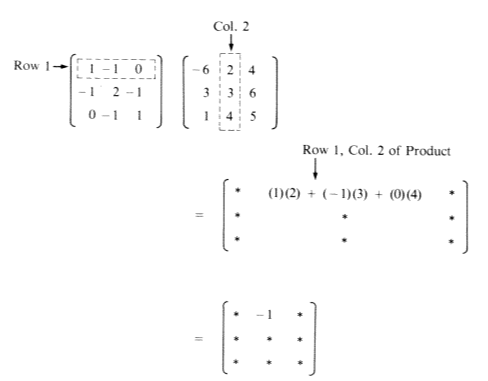
\includegraphics[width=1\linewidth]{images/fig-one-matrix-product-entry.png}
\caption{Computation of one entry in the product of two 3 by 3 matrices
                \label{fig-one-matrix-product-entry}}
\end{figure}
\par
The computation of a product 
can take a considerable amount of time in comparison to the time required to add two matrices. Suppose that \(A\) and \(B\) are \(n\times n\) matrices; then \((A B)_{ij}\) is determined performing \(n\) multiplications and \(n-1\) additions. The full product takes \(n^3\) multiplications and \(n^3 - n^2\) additions. This compares with \(n^2\) additions for the sum of two \(n\times n\) matrices. The product of two 10 by 10 matrices will require 1,000 multiplications and 900 additions, clearly a job that you would assign to a computer. The sum of two matrices requires a more modest 100 additions. This analysis is based on the assumption that matrix multiplication will be done using the formula that is given in the definition. There are more advanced methods that, in theory, reduce operation counts. For example, Strassen's algorithm (\href{https://en.wikipedia.org/wiki/Strassen_algorithm}{https://en.wikipedia.org/wiki/Strassen\_algorithm}) computes the product of two \(n\) by \(n\) matrices in \(7\cdot 7^{\log _2n}-6\cdot  4^{\log _2n}\approx  7 n^{2.808}\) operations. There are practical issues involved in actually using the algorithm in many situations.  For example, round-off error can be more of a problem than with the standard formula. %
\begin{example}[A Matrix Product]\label{ex-matrix-product}
  Let \(A =\left(
\begin{array}{cc}
 1 & 0 \\
 3 & 2 \\
 -5 & 1 \\
\end{array}
\right)\), a \(3\times 2\) matrix, an let \(B =\left(
\begin{array}{c}
 6 \\
 1 \\
\end{array}
\right)\), a \(2\times 1\) matrix. Then \(A B\) is a \(3 \times  1\) matrix:
\begin{equation*}(A B = \left(
\begin{array}{cc}
 1 & 0 \\
 3 & 2 \\
 -5 & 1 \\
\end{array}
\right) \left(
\begin{array}{c}
 6 \\
 1 \\
\end{array}
\right) = \left(
\begin{array}{c}
 1\cdot 6+0\cdot 1 \\
 3 \cdot 6 + 2\cdot 1 \\
 -5 \cdot 6 + 1\cdot 1 \\
\end{array}
\right) = \left(
\begin{array}{c}
 6 \\
 20 \\
 -29 \\
\end{array}
\right)\end{equation*}
%
\end{example}
\par
Remarks:%
\par
\leavevmode%
\begin{enumerate}[label=\arabic*]
\item\hypertarget{li-3}{} The product \(A B\) is defined only if \(A\) is an \(m\times n\) matrix and \(B\) is an \(n\times p\) matrix; that is, the two ``inner'' numbers must be the equal. Furthermore, the order of the product matrix \(A B\) is the ``outer'' numbers, in
this case \(m\times p\).
%
\item\hypertarget{li-4}{}It is wise to first determine the order of a product matrix. For example, if \(A\) is a \(3\times 2\) matrix and \(B\) is a \(2\times 2\) matrix, then \(A B\) is a \(3\times 2\) matrix of the form

\[A B =\left(
\begin{array}{cc}
 c_{11} & c_{12} \\
 c_{21} & c_{22} \\
 c_{31} & c_{32} \\
\end{array}
\right)\] 

Then to obtain, for example, \(C_{31}\), we multiply corresponding entries in the third row of \(A\) times the first column of \(B\)
and add the results.%
\end{enumerate}
%
\begin{example}[Multiplication with a diagonal matrix]\label{ex-diagonal-product}


Let \(A =\left(
\begin{array}{cc}
 -1 & 0 \\
 0 & 3 \\
\end{array}
\right)\), and \(B =\left(
\begin{array}{cc}
 3 & 10 \\
 2 & 1 \\
\end{array}
\right)\) . Then

\(A B =\left(
\begin{array}{cc}
 -1\cdot 3 + 0\cdot 2 & -1\cdot 10+0\cdot 1 \\
 0\cdot 3+3\cdot 2 & 0\cdot 10+3\cdot 1 \\
\end{array}
\right)= \left(
\begin{array}{cc}
 -3 & -10 \\
 6 & 3 \\
\end{array}
\right)\)
%
\par
The net effect is to multiply the first row of \(B\) by -1 and the second row of \(B\) by 3.%
\par
Note: \(B A =\left(
\begin{array}{cc}
 -3 & 30 \\
 -	2 & 3 \\
\end{array}
\right) \neq A B\).   The columns of \(B\) are multiplied by -1 and 3 when the order is switched.
%
\end{example}
\par
Remarks:%
\par
\leavevmode%
\begin{itemize}[label=\textbullet]
\item{} An \(n\times n\) matrix is called a \emph{square matrix}.%
\item{} If \(A\) is a square matrix, \(A A\) is defined and is denoted by \(A^2\) , and \(A A A = A^3\), etc. %
\item{} The \(m\times n\) matrices whose entries are all 0 are denoted by \(\pmb{0}_{m\times n}\), or simply \(\pmb{ 0}\), when no confusion arises regarding the order.\label{notation-1}
%
\end{itemize}
%
\typeout{************************************************}
\typeout{Exercises 1.1.4 Exercises}
\typeout{************************************************}
\subsection[Exercises]{Exercises}\label{exercises-5-1}
\hypertarget{exercisegroup-1}{}\typeout{************************************************}
\typeout{Introduction  }
\typeout{************************************************}
A Exercises%
\begin{exercisegroup}
\item[1.]\hypertarget{exercise-1}{}Let \(A=\left(
\begin{array}{cc}
 1 & -1 \\
 2 & 3 \\
\end{array}
\right)\), \(B =\left(
\begin{array}{cc}
 0 & 1 \\
 3 & -5 \\
\end{array}
\right)\) , and \(C=\left(
\begin{array}{ccc}
 0 & 1 & -1 \\
 3 & -2 & 2 \\
\end{array}
\right)\) %
\par
\leavevmode%
\begin{enumerate}[label=\alph*]
\item\hypertarget{li-8}{} Compute \(A B\) and \(B A\).%
\item\hypertarget{li-9}{} Compute \(A + B\) and \(B + A\).%
\item\hypertarget{li-10}{} If \(c = 3\), show that \(c(A + B) = c A + c B\).%
\item\hypertarget{li-11}{} Show that \((A B)C = A(B C)\).%
\item\hypertarget{li-12}{} Compute \(A^2 C\).%
\item\hypertarget{li-13}{}  Compute \(B + \pmb{0}\)%
\item\hypertarget{li-14}{} Compute \(A \pmb{0}_{2\times 2}\) and \(\pmb{0}_{2\times 2} A\), where \(\pmb{0}_{2\times 2}\) is the \(2\times 2\) zero matrix%
\item\hypertarget{li-15}{} Compute \(0A\), where 0 is the real number (scalar) zero.%
\item\hypertarget{li-16}{} Let \(c = 2\) and \(d = 3\). Show that\((c + d)A = c A + d A\).%
\end{enumerate}
%
\par\smallskip
\par\smallskip
\noindent\textbf{Answer.}\hypertarget{answer-1}{}\quad
 For parts c, d and i of this exercise, only a verification is needed. Here, we supply the result that will appear on both sides of the equality.%
\par
\leavevmode%
\begin{multicols}{1}
\begin{enumerate}[label=\alph*]
\item\hypertarget{li-17}{}  \(AB=\left(
\begin{array}{cc}
 -3 &6 \\
 9 & -13 \\
\end{array}
\right) \quad BA=\left(
\begin{array}{cc}
 2 & 3 \\
 -7 & -18 \\
\end{array}
\right)\)  %
\item\hypertarget{li-18}{}  \(\left(
\begin{array}{cc}
 1 & 0 \\
 5 & -2 \\
\end{array}
\right)\)%
\item\hypertarget{li-19}{} \(\left(
\begin{array}{cc}
 3 & 0 \\
 15 & -6 \\
\end{array}
\right)\)%
\item\hypertarget{li-20}{} \(\left(
\begin{array}{ccc}
 18 & -15 & 15 \\
 -39 & 35 & -35 \\
\end{array}
\right)\)%
\item\hypertarget{li-21}{} \(\left(
\begin{array}{ccc}
 -12 & 5 & -5 \\
 5 & -25 & 25 \\
\end{array}
\right)\)%
\item\hypertarget{li-22}{}\(B+0=B\)%
\item\hypertarget{li-23}{}\(\left(
\begin{array}{cc}
 0 & 0 \\
 0 & 0 \\
\end{array}
\right)\) %
\item\hypertarget{li-24}{}  \(\left(
\begin{array}{cc}
 0 & 0 \\
 0 & 0 \\
\end{array}
\right)\) %
\item\hypertarget{li-25}{}  \(\left(
\begin{array}{cc}
 5 & -5 \\
 10 & 15 \\
\end{array}
\right)\)%
\end{enumerate}
\end{multicols}
%
\item[2.]\hypertarget{exercise-2}{} Let \(A = \left(
\begin{array}{ccc}
 1 & 0 & 2 \\
 2 & -1 & 5 \\
 3 & 2 & 1 \\
\end{array}
\right)\) , \(B =\left(
\begin{array}{ccc}
 0 & 2 & 3 \\
 1 & 1 & 2 \\
 -1 & 3 & -2 \\
\end{array}
\right)\) , and \(C=\left(
\begin{array}{cccc}
 2 & 1 & 2 & 3 \\
 4 & 0 & 1 & 1 \\
 3 & -1 & 4 & 1 \\
\end{array}
\right)\)
Compute, if possible;%
\par
\leavevmode%
\begin{multicols}{2}
\begin{enumerate}[label=\alph*]
\item\hypertarget{li-26}{} \(A - B\)%
\item\hypertarget{li-27}{} \(A B\) %
\item\hypertarget{li-28}{} \(A C - B C\) %
\item\hypertarget{li-29}{} \(A(B C)\)%
\item\hypertarget{li-30}{} \(C A - C B\)%
\item\hypertarget{li-31}{} \(C \left(
\begin{array}{c}
 x \\
 y \\
 z \\
 w \\
\end{array}
\right)\)%
\end{enumerate}
\end{multicols}
%
\par\smallskip
\item[3.]\hypertarget{exercise-3}{} Let \(A =\left(
\begin{array}{cc}
 2 & 0 \\
 0 & 3 \\
\end{array}
\right)\) . Find a matrix B such that \(A B = I\) and \(B A = I\), where \(I = \left(
\begin{array}{cc}
 1 & 0 \\
 0 & 1 \\
\end{array}
\right)\)%
\par\smallskip
\par\smallskip
\noindent\textbf{Answer.}\hypertarget{answer-2}{}\quad
  \(\left(
\begin{array}{cc}
 1/2 & 0 \\
 0 & 1/3 \\
\end{array}
\right)\)
%
\item[4.]\hypertarget{exercise-4}{} Find \(A I\) and \(B I\) where \(I\) is as in Exercise 3, where
\(A = \left(
\begin{array}{cc}
 1 & 8 \\
 9 & 5 \\
\end{array}
\right)\) and \(B = \left(
\begin{array}{cc}
 -2 & 3 \\
 5 & -7 \\
\end{array}
\right)\). 
 What do you notice?%
\par\smallskip
\item[5.]\hypertarget{exercise-5}{} Find \(A^3\) if \(A=\left(
\begin{array}{ccc}
 1 & 0 & 0 \\
 0 & 2 & 0 \\
 0 & 0 & 3 \\
\end{array}
\right)\) . What is \(A^{15}\) equal to?
%
\par\smallskip
\par\smallskip
\noindent\textbf{Answer.}\hypertarget{answer-3}{}\quad
  \(A^3=\left(
\begin{array}{ccc}
 1 & 0 & 0 \\
 0 & 8 & 0 \\
 0 & 0 & 27 \\
\end{array}
\right)\)  \(A^{15}=\left(
\begin{array}{ccc}
 1 & 0 & 0 \\
 0 & 32768 & 0 \\
 0 & 0 & 14348907 \\
\end{array}
\right)\)
%
\end{exercisegroup}
\par\smallskip\noindent
\hypertarget{exercisegroup-2}{}\typeout{************************************************}
\typeout{Introduction  }
\typeout{************************************************}
B Exercises%
\begin{exercisegroup}
\item[6.]\hypertarget{exercise-6}{}\leavevmode%
\begin{enumerate}[label=\alph*]
\item\hypertarget{li-32}{} Determine \(I^2\) and \(I^3 \text{if}\) \(I = \left(
\begin{array}{ccc}
 1 & 0 & 0 \\
 0 & 1 & 0 \\
 0 & 0 & 1 \\
\end{array}
\right)\).%
\item\hypertarget{li-33}{} What is \(I^n\) equal to for any \(n\geq 1\)?%
\item\hypertarget{li-34}{} Prove your answer to part (b) by induction.%
\end{enumerate}
%
\par\smallskip
\item[7.]\hypertarget{exercise-7}{}\leavevmode%
\begin{enumerate}[label=\alph*]
\item\hypertarget{li-35}{}If \(A =\left(
\begin{array}{cc}
 2 & 1 \\
 1 & -1 \\
\end{array}
\right)\), \(X =\left(
\begin{array}{c}
 x_1 \\
 x_2 \\
\end{array}
\right)\), and \(B =\left(
\begin{array}{c}
 3 \\
 1 \\
\end{array}
\right)\) , show that \(A X =B\) is a way of expressing the system  
    \(2x_1 + x_2 = 3\\ \\ x_1 - x_2= 1\)  using matrices.%
\item\hypertarget{li-36}{} Express the following systems of equations using matrices:%
\par
%
\begin{multicols}{2}
\begin{enumerate}[label=\roman*]
\item\hypertarget{li-37}{}  \(2 x_1- x_2= 4\\
				\\
				\text{   }x_1+ x_2= 0\)%
\item\hypertarget{li-38}{}  \(x_1+ x_2+ 2 x_3= 1\\
				\\
				x_1+ 2 x_2-x_3= -1\\
				\\
				x_1+ 3 x_2+x_3= 5\)%
\item\hypertarget{li-39}{}  \(x_1+x_2\text{             }= 3\\
				\\
				\text{          }x_2\text{              }= 5\\
				\\
				x_1\text{         }+ 3x_3= 6\)
				%
\end{enumerate}
\end{multicols}

%
\end{enumerate}
%
\par\smallskip
\par\smallskip
\noindent\textbf{Answer.}\hypertarget{answer-4}{}\quad
\leavevmode%
\begin{enumerate}[label=\alph*]
\item\hypertarget{li-40}{} \(Ax=\left(
\begin{array}{c}
 2x_1+1x_2 \\
 1x_1-1x_2 \\
\end{array}
\right)\) equals \(\left(
\begin{array}{c}
 3 \\
 1 \\
\end{array}
\right)\) if and only if both of the equalities 
     \(2x_1+x_2=3 \textrm{ and } x_1-x_2=1\) are true.%
\item\hypertarget{li-41}{} (i)  \(A=\left(
\begin{array}{cc}
 2 & -1 \\
 1 & 1 \\
\end{array}
\right)\)   \(x=\left(
\begin{array}{c}
 x_1 \\
 x_2 \\
\end{array}
\right)\)   \(B=\left(
\begin{array}{c}
 4 \\
 0 \\
\end{array}
\right)\)
%
\item\hypertarget{li-42}{}  \(A=\left(
\begin{array}{ccc}
 1 & 1 & 2 \\
 1 & 2 & -1 \\
 1 & 3 & 1 \\
\end{array}
\right)\) \(x=\left(
\begin{array}{c}
 x_1 \\
 x_2 \\
 x_3 \\
\end{array}
\right)\)   \(B=\left(
\begin{array}{c}
 1 \\
 -1 \\
 5 \\
\end{array}
\right)\)
%
\item\hypertarget{li-43}{}   \(A=\left(
\begin{array}{ccc}
 1 & 1 & 0 \\
 0 & 1 & 0 \\
 1 & 0 & 3 \\
\end{array}
\right)\)  \(x=\left(
\begin{array}{c}
 x_1 \\
 x_2 \\
 x_3 \\
\end{array}
\right)\)    \(B=\left(
\begin{array}{c}
 3 \\
 5 \\
 6 \\
\end{array}
\right)\)
%
\end{enumerate}
%
\end{exercisegroup}
\par\smallskip\noindent
\typeout{************************************************}
\typeout{Section 1.2 Special Types of Matrices}
\typeout{************************************************}
\section[Special Types of Matrices]{Special Types of Matrices}\label{s-special-matrices}
We have already investigated, in exercises in the previous section, one special type of matrix. That was the  zero matrix, and found that it behaves in matrix algebra 
in an analogous fashion to the real number 0; that is, as the additive identity. We will now investigate the properties of a few other special matrices.%
\begin{definition}[Diagonal Matrix]\label{def-diagonal-matrix}
A square matrix D is called a diagonal matrix if \(d_{i j}\) = 0 whenever \(i \neq  j\).%
\end{definition}
\begin{example}[Some diagonal matrices]\label{example-diagonal-matrices}
   \(A = \left(
\begin{array}{ccc}
 1 & 0 & 0 \\
 0 & 2 & 0 \\
 0 & 0 & 5 \\
\end{array}
\right)\), \(B= \left(
\begin{array}{ccc}
 3 & 0 & 0 \\
 0 & 0 & 0 \\
 0 & 0 & -5 \\
\end{array}
\right)\), and \(I = \left(
\begin{array}{ccc}
 1 & 0 & 0 \\
 0 & 1 & 0 \\
 0 & 0 & 1 \\
\end{array}
\right)\) are all diagonal matrices.
%
\end{example}
\par
In the example above, the \(3\times 3\) diagonal matrix \(I\) whose diagonal entries are all 1's has the distinctive property that for any other \(3\times 3\) matrix \(A\) we have \(A I = I A = A\). For example:%
\begin{example}[Multiplying by the Identity Matrix]\label{ex-matrix-identity-product}
If \(A = \left(
\begin{array}{ccc}
 1 & 2 & 5 \\
 6 & 7 & -2 \\
 3 & -3 & 0 \\
\end{array}
\right)\), then

\(A I =\left(
\begin{array}{ccc}
 1 & 2 & 5 \\
 6 & 7 & -2 \\
 3 & -3 & 0 \\
\end{array}
\right)\) and

\(I A = \left(
\begin{array}{ccc}
 1 & 2 & 5 \\
 6 & 7 & -2 \\
 3 & -3 & 0 \\
\end{array}
\right)\).
%
\end{example}
\par
In other words, the matrix \(I\) behaves in matrix algebra like the real number 1; that is, as a multiplicative identity. In matrix algebra, the matrix \(I\) is called simply the identity matrix. Convince yourself that if A is any \(n\times n\) matrix \(A I = I A = A\).%
\begin{definition}[Identity Matrix]\label{def-identity-matrix}
\index{Identity Matrix}\label{notation-2}
The \(n\times n\) diagonal matrix \(I_n\) whose 
diagonal components are all 1's is called the identity matrix.  If the context is clear, simply \(I\).%
\end{definition}
\par
In the set of real numbers we recall that, given a nonzero real number \(x\), there exists a real number \(y\) such that \(x y = y x
=1\). We know that real numbers commute under multiplication so that the two equations can be summarized as \(x y = 1\). Further we know that \(y =x^{-1}= \frac{1}{x}\). Do we have an analogous situation in \(M_{n\times n}(\mathbb{R})\)? Can we define the multiplicative inverse of an \(n\times n\) matrix \(A\)? It seems natural to imitate the definition of multiplicative inverse in the real numbers.%
\begin{definition}[Matrix Inverse]\label{def-matrix-inverse}
\index{Inverse!Matrix}\label{notation-3}
Let A be an \(n\times n\) matrix. If there exists 
an \(n\times n\) matrix B such that \(A B = B A =I\), then B is a multiplicative inverse of A (called simply an inverse of A) and is denoted by \(A^{-1}\)%
\end{definition}
\par
When we are doing computations involving matrices, it would be helpful to know that when we find \(A^{-1}\), the answer we 
obtain is the only inverse of the given matrix.  This would let us refer to \emph{the} inverse of a matrix.  We refrained from saying that in the definition, but the theorem below justifies it. %
\par
Remark: Those unfamiliar with the laws of matrices should go over the proof of Theorem 5.4.1 after they have familiarized themselves with the Laws of Matrix Algebra in Section 5.5.%
\begin{theorem}[Inverses are unique]\label{theorem-unique-inverse}
The inverse of an \(n\times n\) matrix A, when it exists, is unique.%
\end{theorem}
\begin{proof}\hypertarget{proof-1}{}
Let \(A\) be an \(n\times n\) matrix. Assume to the contrary, that \(A\) has two (different) inverses, say \(B\) and \(C\). Then
\begin{equation*}
\begin{split}
B &= B I  & \textrm{ Identity property of } I\\
& =B (A  ) & \textrm{ Assumption that } C \textrm{ is an inverse of } A\\
& = (B A) C & \textrm{ Associativity of matrix multiplication}\\
& = I C  & \textrm{ Assumption that } B \textrm{ is an inverse of } A\\
& = C & \textrm{ Identity property of } I
\end{split}
\end{equation*}%
\end{proof}
\par
Let \(A =\left(
\begin{array}{cc}
 2 & 0 \\
 0 & 3  \\
\end{array}
\right)\) .  What is \(A^{-1}\) ? Without too much difficulty, by trial and error, we determine that \(A^{-1}= \left(
\begin{array}{cc}
 \frac{1}{2} & 0 \\
 0 & \frac{1}{3} \\
\end{array}
\right)\) . This might lead us to guess that the inverse is found by taking the reciprocal of all nonzero entries of a matrix. Alas, it isn't
that easy!%
\par
If \(A =\left(
\begin{array}{cc}
 1 & 2 \\
 -3 & 5 \\
\end{array}
\right)\) , the ``reciprocal rule'' would tell us that the inverse of \(A\) is \(B=\left(
\begin{array}{cc}
 1 & \frac{1}{2} \\
 \frac{-1}{3} & \frac{1}{5} \\
\end{array}
\right)\). Try computing \(A B\) and you will see that you don't get the identity matrix.  So, what \emph{is} \(A^{-1}\)? In order to understand more completely the notion of the inverse of a matrix, it would be beneficial to have a formula that would enable us to compute the inverse of at least a \(2\times 2\) matrix. To do this, we introduce the definition of the determinant of a \(2\times 2\) matrix. Appendix A gives a more complete description of the determinant of a \(2\times 2\) and higher-order matrices.%
\begin{definition}[Determinant of a 2 by 2 Matrix]\label{determinant-2by2}
\label{notation-4}
 Let \(A =\left(
\begin{array}{cc}
 a & b \\
 c & d \\
\end{array}
\right)\). The determinant of A is the number \(\det  A = a d - b c\).%
\end{definition}
\par
In addition to \(\det  A\), common notation for the determinant of matrix \(A\)is \(\lvert A \rvert\).  This is particularly common when writing outthe whole matrix, which case we would write \(\left|
\begin{array}{cc}
 a & b \\
 c & d \\
\end{array}
\right|\) for the determinant of the general \(2 \times 2\) matrix.%
\begin{example}[Some Determinants of two by two matrices]\label{ex-some-determinants}
If \(A =\left(
\begin{array}{cc}
 1 & 2 \\
 -3 & 5 \\
\end{array}
\right)\)  then \(\det  A = 1\cdot 5 -2\cdot  (-3)=11\). 

If \(B =\left(
\begin{array}{cc}
 1 & 2 \\
 2 & 4 \\
\end{array}
\right)\)  then \(\det  B = 1\cdot 4 -2\cdot 2=0\)
%
\end{example}
\begin{theorem}[Inverse of 2 by 2 Matrix]\label{theorem-inverse-two-by-two}
 Let \(A =\left(
\begin{array}{cc}
 a & b \\
 c & d \\
\end{array}
\right)\).  If \(\det  A\neq  0\), then \(A^{-1} =\frac{1}{\det  A}\left(
\begin{array}{cc}
 d & -b \\
 -c & a \\
\end{array}
\right)\)%
\end{theorem}
\begin{proof}\hypertarget{proof-2}{}
See Exercise 4 at the end of this section.%
\end{proof}
\begin{example}[Finding Inverses]\label{ex-finding-inverses}
Can we find the inverses of the matrices in \hyperref[ex-some-determinants]{Example~\ref{ex-some-determinants}}? 

If \(A =\left(
\begin{array}{cc}
 1 & 2 \\
 -3 & 5 \\
\end{array}
\right)\)  then 
\begin{equation*}A^{-1}= \frac{1}{11}\left(
\begin{array}{cc}
 5 & -2 \\
 3 & 1 \\
\end{array}
\right)=\left(
\begin{array}{cc}
 \frac{5}{11} & -\frac{2}{11} \\
 \frac{3}{11} & \frac{1}{11} \\
\end{array}
\right)\end{equation*}

The reader should verify that \(A A^{-1}=A^{-1}A = I\).%
\par
The second matrix, \(B\) has a determinant equal to zero. We we tried to apply the formula in \hyperref[theorem-inverse-two-by-two]{Theorem~\ref{theorem-inverse-two-by-two}}, we would be dividing by zero.
For this reason, the formula can't be applied and in fact \(B^{-1}\) does not exist. 
%
\end{example}
\par
Remarks:%
\par
\leavevmode%
\begin{itemize}[label=\textbullet]
\item{} In general, if \(A\) is a \(2\times 2\) matrix and if \(\det  A = 0\), then \(A^{-1}\) does not exist.%
\item{} A formula for the inverse of \(n\times n\) matrices \(n\geq  3\) can be derived that also involves \(\det  A\), Hence, in general, if the determinant of a matrix is zero, the matrix does not have an inverse. However the formula for even a \(3 \times  3\) matrix is very long and is not the most efficient way to compute the inverse of a matrix.%
\item{} In Chapter 12 we will develop a technique to compute the inverse of a higher-order matrix, if it exists.%
\item{} Matrix inversion comes first in the hierarchy of matrix operations; therefore, \(A B^{-1}\) is \(A (B^{-1})\).%
\end{itemize}
%
\typeout{************************************************}
\typeout{Exercises 1.2.1 Exercises}
\typeout{************************************************}
\subsection[Exercises]{Exercises}\label{exercises-5-4}
\hypertarget{exercisegroup-3}{}\typeout{************************************************}
\typeout{Introduction  }
\typeout{************************************************}
A Exercises%
\begin{exercisegroup}
\item[1.]\hypertarget{exercise-8}{} For the given matrices \(A\) find \(A^{-1}\) if it exists and verify that \(A A^{-1}=A^{-1}A = I\).  If \(A^{-1}\) does not exist
explain why.%
\par
\leavevmode%
\begin{enumerate}[label=\alph*]
\item\hypertarget{li-48}{}  \(A = \left(
\begin{array}{cc}
 1 & 3 \\
 2 & 1 \\
\end{array}
\right)\) 
%
\item\hypertarget{li-49}{} \(A=\left(
\begin{array}{cc}
 6 & -3 \\
 8 & -4 \\
\end{array}
\right)\)
%
\item\hypertarget{li-50}{} \(A = \left(
\begin{array}{cc}
 1 & -3 \\
 0 & 1 \\
\end{array}
\right)\)
%
\item\hypertarget{li-51}{}  \(A = \left(
\begin{array}{cc}
 1 & 0 \\
 0 & 1 \\
\end{array}
\right)\)
%
\item\hypertarget{li-52}{} Use the definition of the inverse of a matrix to find \(A^{-1}\):
 \(A=\left(
\begin{array}{ccc}
 3 & 0 & 0 \\
 0 & \frac{1}{2} & 0 \\
 0 & 0 & -5 \\
\end{array}
\right)\)
%
\end{enumerate}
%
\par\smallskip
\par\smallskip
\noindent\textbf{Answer.}\hypertarget{answer-5}{}\quad
\leavevmode%
\begin{multicols}{2}
\begin{enumerate}[label=\alph*]
\item\hypertarget{li-53}{} \(\left(
\begin{array}{cc}
 -1/5 & 3/5 \\
 2/5 & -1/5 \\
\end{array}
\right)\)%
\item\hypertarget{li-54}{} \(\left(
\begin{array}{cc}
 1 & 3 \\
 0 & 1 \\
\end{array}
\right)\) %
\item\hypertarget{li-55}{}  No inverse exists.%
\item\hypertarget{li-56}{} \(A^{-1}=A\)   %
\item\hypertarget{li-57}{} \(\left(
\begin{array}{ccc}
 1/3 & 0 & 0 \\
 0 & 2 & 0 \\
 0 & 0 & -1/5 \\
\end{array}
\right)\)
%
\end{enumerate}
\end{multicols}
%
\item[2.]\hypertarget{exercise-9}{} For the given matrices \(A\) find \(A^{-1}\) if it exists and verify that \(A A^{-1}=A^{-1}A = I\) If \(A^{-1}\) does not exist
explain why.%
\par
\leavevmode%
\begin{enumerate}[label=\alph*]
\item\hypertarget{li-58}{} \(A =\left(
\begin{array}{cc}
 2 & -1 \\
 -1 & 2 \\
\end{array}
\right)\)
%
\item\hypertarget{li-59}{} \(A = \left(
\begin{array}{cc}
 0 & 1 \\
 0 & 2 \\
\end{array}
\right)\)
%
\item\hypertarget{li-60}{}  \(A= \left(
\begin{array}{cc}
 1 & c \\
 0 & 1 \\
\end{array}
\right)\)
%
\item\hypertarget{li-61}{}  \(A = \left(
\begin{array}{cc}
 a & b \\
 b & a \\
\end{array}
\right)\), were \(a > b>0\).
%
\end{enumerate}
%
\par\smallskip
\item[3.]\hypertarget{prob-5-2-3}{}\leavevmode%
\begin{enumerate}[label=\alph*]
\item\hypertarget{li-62}{} Let \(A = \left(
\begin{array}{cc}
 2 & 3 \\
 1 & 4 \\
\end{array}
\right)\) and \(B =\left(
\begin{array}{cc}
 3 & -3 \\
 2 & 1 \\
\end{array}
\right)\). Verify that \((A B)^{-1}= B^{-1}A^{-1}\) . 
%
\item\hypertarget{li-63}{} Let \(A\) and \(B\) be \(n\times n\) invertible matrices. Prove that \((A B)^{-1}= B^{-1}A^{-1}\). Why is the right side of the above statement written ``backwards''? Is this necessary? Hint: Use \hyperref[theorem-unique-inverse]{Theorem~\ref{theorem-unique-inverse}}%
\end{enumerate}
%
\par\smallskip
\par\smallskip
\noindent\textbf{Answer.}\hypertarget{answer-6}{}\quad
 Let A and B be \(n\) by \(n\) invertible matrices.%
\par

\begin{equation*}
\begin{split}
\left(B^{-1}A^{-1}\right)(AB)&=\left(B^{-1}\right)\left(A^{-1}(AB)\right)\\
   &= \left(B^{-1}\right) \left(\left(A^{-1} A\right) B\right)\\
   &=(\left(B^{-1}\right)I B )\\
    &=B^{-1}(B)\\
    &=I 
\end{split}
\end{equation*}
%
\par
Similarly, \((AB)\left(B^{-1}A^{-1}\right)=I\).%
\par
By \hyperref[theorem-unique-inverse]{Theorem~\ref{theorem-unique-inverse}}, \(B^{-1}A^{-1}\) is the only inverse of \(AB\). If we tried to invert \(AB\) with \(A^{-1}B^{-1}\), we would be unsuccessful since we cannot rearrange the order of the matrices. %
\end{exercisegroup}
\par\smallskip\noindent
\hypertarget{exercisegroup-4}{}\typeout{************************************************}
\typeout{Introduction  }
\typeout{************************************************}
B Exercises%
\begin{exercisegroup}
\item[4.]\hypertarget{exercise-11}{} Let Let \(A =\left(
\begin{array}{cc}
 a & b \\
 c & d \\
\end{array}
\right)\). Derive the formula for \(A^{-1}\).%
\par\smallskip
\item[5.]\hypertarget{prob-5-2-5}{}(Linearity of Determinants)\space\space{}\leavevmode%
\begin{enumerate}[label=\alph*]
\item\hypertarget{li-64}{}Let \(A\) and \(B\) be as in \hyperlink{prob-5-2-3}{Exercise~1.2.1.3}. Show that \(\det (A B) =(\det  A)(\det  B)\).
%
\item\hypertarget{li-65}{} It can be shown that the statement in part (a) is true for all \(n\times n\) matrices. Let \(A\) be any invertible \(n\times n\) matrix. Prove that \(\det \left(A^{-1}\right) =(\det  A)^{-1}\). Note: The determinant of the identity matrix \(I_n\) is 1 for all \(n\).
%
\item\hypertarget{li-66}{} Verify that the equation in part (b) is true for the matrix in exercise l(a) of this section.
%
\end{enumerate}
%
\par\smallskip
\par\smallskip
\noindent\textbf{Answer.}\hypertarget{answer-7}{}\quad
 \(1=\det  I=\det \left(AA^{-1}\right)=\det  A\text{  }\det  A^{-1}\). Now solve for \(\det  A^{-1}\). 
%
\item[6.]\hypertarget{exercise-13}{} Prove by induction that for \(n \geq 1\), \(\left(
\begin{array}{cc}
 a & 0 \\
 0 & b \\
\end{array}
\right)^n= \left(
\begin{array}{cc}
 a^n & 0 \\
 0 & b^n \\
\end{array}
\right)\).
%
\par\smallskip
\item[7.]\hypertarget{exercise-14}{} Use the assumptions in \hyperlink{prob-5-2-5}{Exercise~1.2.1.5} to prove by induction that if \(n \geq 1\), \(\det \left(A^n\right) = (\det  A)^n\).%
\par\smallskip
\par\smallskip
\noindent\textbf{Answer.}\hypertarget{answer-8}{}\quad
Basis: \((n=1): \det  A^1=\det  A =(\det  A )^1\)%
\par
Induction: Assume \(\det  A^n=(\det  A)^n\) for some \(n\geq 1\).%
\par

\begin{equation*}
\begin{split}
 \det  A^{n+1} & =\det \left(A^nA\right)\quad \textrm{ by the definition of exponents}\\
   &=\det \left(A^n\right)\det (A)\quad \textrm{ by exercise 5} \\
   &=det  A)^n(\det  A)\quad \textrm{ by the induction hypothesis }\\
  &=(\det  A)^{n+1}
\end{split}
\end{equation*}
%
\item[8.]\hypertarget{exercise-15}{}Prove: If the determinant of a matrix \(A\) is zero, then \(A\) does not have an inverse. Hint: Use the indirect method of proof and exercise 5.%
\par\smallskip
\end{exercisegroup}
\par\smallskip\noindent
\hypertarget{exercisegroup-5}{}\typeout{************************************************}
\typeout{Introduction  }
\typeout{************************************************}
C Exercises%
\begin{exercisegroup}
\item[9.]\hypertarget{exercise-16}{}\leavevmode%
\begin{enumerate}[label=\alph*]
\item\hypertarget{li-67}{} Let \(A, B, \textrm{ and } D\) be \(n\times n\) matrices. Assume that \(B\) is invertible. If \(A = B D B^{-1}\) , prove by induction
that \(A^m= B D^m B^{-1}\) is true for \(m \geq  1\).%
\item\hypertarget{li-68}{}Given that \(A = \left(
\begin{array}{cc}
 -8 & 15 \\
 -6 & 11 \\
\end{array}
\right) = B \left(
\begin{array}{cc}
 1 & 0 \\
 0 & 2 \\
\end{array}
\right) B^{-1}\) where \(B=\left(
\begin{array}{cc}
 5 & 3 \\
 3 & 2 \\
\end{array}
\right)\) what is \(A^{10}\)?%
\end{enumerate}
%
\par\smallskip
\par\smallskip
\noindent\textbf{Answer.}\hypertarget{answer-9}{}\quad
\leavevmode%
\begin{enumerate}[label=\alph*]
\item\hypertarget{li-69}{} Assume \(A=B D B^{-1}\)%
\par
Basis:  \((m=1\)): \(A^{1}=A=B D^1 B^{-1} \) is given.%
\par
Induction: Assume that for some positive integer \(m\), \(A^m=BD^mB^{-1}\)%
\par
\begin{equation*}
\begin{split}
A^{m+1} &=A^mA\\
 &=(B D^m B^{-1})(BDB^{-1})\quad \textrm{ by the induction hypothesis} \\
 &=(BD^m(B^{-1} B ) (DB^{-1}) \quad \textrm{ by associativity} \\
 &=B D^m  D B^{-1}  \quad \textrm{ by the definition of inverse}\\
 &=B D^{m+1} B^{-1} \quad \square
\end{split}
\end{equation*}
%
\item\hypertarget{li-70}{} \(A^{10}=BD^{10}B^{-1}= \left(
\begin{array}{cc}
 -9206 & 15345 \\
 -6138 & 10231 \\
\end{array}
\right)\)%
\end{enumerate}
%
\end{exercisegroup}
\par\smallskip\noindent
\typeout{************************************************}
\typeout{Section 1.3 Laws of Matrix Algebra}
\typeout{************************************************}
\section[Laws of Matrix Algebra]{Laws of Matrix Algebra}\label{s-laws-of-matrix-algebra}
\index{Laws of Matrix Algebra}The following is a summary of the basic laws of matrix operations. Assume that the indicated operations are defined; that is, that the orders of the matrices \(A\), \(B\) and \(C\) are such that the operations make sense.%
\leavevmode%
\begin{table}
\centering
\begin{tabular}{ccc}
(1)&Communtative Law of Addition&\(A + B = B + A\)\tabularnewline[0pt]
(2)&Associative Law of Addition&\(A + (B + C) = (A + B) + C\)\tabularnewline[0pt]
(3)&Distrutive Law of a Scalar over Matrices &\(c(A + B) = c A + c B\), where \(c \in  \mathbb{R}\).\tabularnewline[0pt]
(4)&Distrutive Law of Scalars over a Matrix &\(\left(c_1 + c_2 \right)A = c_1A +c_2 A\), where \(c_1, c_2 \in  \mathbb{R}\).\tabularnewline[0pt]
(5)&Associative Law of Scalar Multiplication&\(c_1 \left(c_2 A\right) =\left(c_1 \cdot c_2 \right)A\), where \(c_1, c_2 \in  \mathbb{R}\).\tabularnewline[0pt]
(6)&Zero Matrix Annihilates all Products&\(\pmb{0}A = \pmb{0}\), where \pmb{ 0} is the zero matrix.\tabularnewline[0pt]
(7)&Zero Scalar Annihilates all Products &\(0 A =\pmb{0}\), where 0 on the left is the scalar zero.\tabularnewline[0pt]
(8)&Zero Matrix is an identity for Addition&\(A + 0 = A\). \tabularnewline[0pt]
(9)&Negation produces additive inverses&\(A + (-1)A = \pmb{0}\). \tabularnewline[0pt]
(10)&Right Distrutive Law of Matrix Multiplication&\(A(B + C) = A B + A C\). \tabularnewline[0pt]
(11)&Left  Distrutive Law of Matrix Multiplication&\((B + C)A = B A + C A\). \tabularnewline[0pt]
(12)&Associative Law of Multiplication&\(A(B C) = (A B)C\).\tabularnewline[0pt]
(13)&Identity Matrix is a Multiplicative Identity&\(I A = A\) and \(A I = A\).\tabularnewline[0pt]
(14)&Involution Property of Inverses&If \(A^{-1}\) exists,\(\left(A^{-1} \right)^{-1} = A\).\tabularnewline[0pt]
(15)&Inverse of Product Rule&If \(A^{-1}\) and \(B^{-1}\) exist, \((A B)^{-1}= B^{-1}A^{-1}\) 
\end{tabular}
\caption{Laws of Matrix Algebra\label{table-matrix-laws}}
\end{table}
\begin{example}[More Precise Statement of one Law]\label{ex-statement-precise}
 If we wished to write out each of the above laws more completely, we would specify the orders of the matrices. For example, Law 10 should read:%
\begin{quote}Let \(A\), \(B\), and \(C\) be \(m\times n\), \(n\times p\), and \(n\times p\) matrices, respectively, then \(A(B + C) = A B + A C\)%
\end{quote}
\end{example}
\par
Remarks:%
\par
\leavevmode%
\begin{itemize}[label=\textbullet]
\item{} Notice the absence of the ``law'' \(A B = B A\). Why? %
\item{} Is it really necessary to have both a right (No. 11) and a left (No. 10) distributive law? Why?%
\end{itemize}

%
\typeout{************************************************}
\typeout{Exercises 1.3.1 Exercises}
\typeout{************************************************}
\subsection[Exercises]{Exercises}\label{exercises-5-5}
\hypertarget{exercisegroup-6}{}\typeout{************************************************}
\typeout{Introduction  }
\typeout{************************************************}
A Exercises%
\begin{exercisegroup}
\item[1.]\hypertarget{exercise-17}{} Rewrite the above laws specifying as in \hyperref[ex-statement-precise]{Example~\ref{ex-statement-precise}} the orders of the matrices.%
\par\smallskip
\par\smallskip
\noindent\textbf{Answer.}\hypertarget{answer-10}{}\quad
\leavevmode%
\begin{enumerate}[label=\alph*]
\item\hypertarget{li-73}{} Let \(A\) and \(B\) be \(m\) by \(n\) matrices. Then \(A+B=B+A\),%
\item\hypertarget{li-74}{} Let \(A\), \(B\), and \(C\) be \(m\) by \(n\) matrices. Then \(A+(B+C)=(A+B)+C\).%
\item\hypertarget{li-75}{} Let \(A\) and \(B\) be \(m\) by \(n\) matrices, and let \(c\in \mathbb{R}\). Then \(c(A+B)=cA+cB\),%
\item\hypertarget{li-76}{} Let \(A\) be an \(m\) by \(n\) matrix, and let \(c_1,c_2\in \mathbb{R}\). Then \(\left(c_1+c_2\right)A=c_1A+c_2A\).%
\item\hypertarget{li-77}{} Let \(A\) be an \(m\) by \(n\) matrix, and let \(c_1,c_2\in \mathbb{R}\). Then \(c_1\left(c_2A\right)=\left(c_1c_2\right)A\)%
\item\hypertarget{li-78}{} Let \(\pmb{0}\) be the zero matrix, of size \(m \textrm{ by } n\), and let \(A\) be a matrix of size \(n \textrm{ by } r\). Then \(\pmb{0}A=\pmb{0}=\textrm{ the } m \textrm{ by } r \textrm{ zero matrix}\).%
\item\hypertarget{li-79}{} Let \(A\) be an \(m \textrm{ by } n\) matrix, and \(0 = \textrm{ the number zero}\). Then \(0A=0=\textrm{ the } m \textrm{ by } n \textrm{ zero matrix}\).%
\item\hypertarget{li-80}{} Let \(A\) be an \(m \textrm{ by } n\) matrix, and let \(\pmb{0}\) be the \(m \textrm{ by } n\) zero matrix. Then \(A+\pmb{0}=A\). %
\item\hypertarget{li-81}{} Let \(A\) be an \(m \textrm{ by } n\) matrix. Then \(A+(- 1)A=\pmb{0}\), where \(\pmb{0}\) is the \(m \textrm{ by } n\) zero matrix.%
\item\hypertarget{li-82}{} Let \(A\), \(B\), and \(C\) be \(m \textrm{ by } n\), \(n \textrm{ by } r\), and \(n \textrm{ by } r\) matrices respectively. Then \(A(B+C)=AB+AC\).%
\item\hypertarget{li-83}{} Let \(A\), \(B\), and \(C\) be \(m \textrm{ by } n\), \(r \textrm{ by } m\), and \(r \textrm{ by } m\) matrices respectively.
 Then \((B+C)A=BA+CA\).%
\item\hypertarget{li-84}{} Let \(A\), \(B\), and \(C\) be \(m \textrm{ by } n\), \(n \textrm{ by } r\), and \(r \textrm{ by } p\) matrices respectively.
 Then \(A(BC)=(AB)C\).%
\item\hypertarget{li-85}{}Let \(A\) be an \(m \textrm{ by } n\) matrix, \(I_m\) the \(m \textrm{ by } m\) identity matrix,
 and \(I_n\) the \(n \textrm{ by } n\) identity matrix. Then \(I_mA=AI_n=A\)%
\item\hypertarget{li-86}{} Let \(A\) be an \(n \textrm{ by } n\) matrix. Then if \(A^{-1}\) exists,
 \(\left(A^{-1}\right)^{-1}=A\).%
\item\hypertarget{li-87}{} Let \(A\) and \(B\) be \(n \textrm{ by } n\) matrices.
 Then if \(A^{-1}\) and \(B^{-1}\) exist, \((AB)^{-1}=B^{-1}A^{-1}\).%
\end{enumerate}
%
\item[2.]\hypertarget{exercise-18}{} Verify each of the Laws of Matrix Algebra using examples.%
\par\smallskip
\item[3.]\hypertarget{exercise-19}{} Let \(A = \left(
\begin{array}{cc}
 1 & 2 \\
 0 & -1 \\
\end{array}
\right)\), \(B= \left(
\begin{array}{ccc}
 3 & 7 & 6 \\
 2 & -1 & 5 \\
\end{array}
\right)\), and \(C= \left(
\begin{array}{ccc}
 0 & -2 & 4 \\
 7 & 1 & 1 \\
\end{array}
\right)\). Compute the following as efficiently as possible by using any of the Laws of Matrix Algebra:%
\par
\leavevmode%
\begin{enumerate}[label=\alph*]
\item\hypertarget{li-88}{} \(A B + A C\)%
\item\hypertarget{li-89}{} \(A^{-1}\)%
\item\hypertarget{li-90}{} \(A(B + C)\)%
\item\hypertarget{li-91}{}  \(\left(A^2\right)^{-1}\)%
\item\hypertarget{li-92}{}  \((C + B)^{-1}A^{-1}\)%
\end{enumerate}
%
\par\smallskip
\par\smallskip
\noindent\textbf{Answer.}\hypertarget{answer-11}{}\quad
\leavevmode%
\begin{enumerate}[label=\alph*]
\item\hypertarget{li-93}{} \(AB+AC=\left(
\begin{array}{ccc}
 21 & 5 & 22 \\
 -9 & 0 & -6 \\
\end{array}
\right)\)%
\item\hypertarget{li-94}{} \(A(B+C)=A B+ B C\)%
\item\hypertarget{li-95}{} \(A^{-1}=\left(
\begin{array}{cc}
 1 & 2 \\
 0 & -1 \\
\end{array}
\right)=A\)%
\item\hypertarget{li-96}{} \(\left(A^2\right)^{-1}=(AA)^{-1}=(A^{-1}A)=I^{-1}=I \quad \) by part c%
\end{enumerate}
%
\item[4.]\hypertarget{exercise-20}{} Let \(A =\left(
\begin{array}{cc}
 7 & 4 \\
 2 & 1 \\
\end{array}
\right)\) and \(B =\left(
\begin{array}{cc}
 3 & 5 \\
 2 & 4 \\
\end{array}
\right)\). Compute the following as efficiently as possible by using any of the Laws of Matrix Algebra:%
\par
\leavevmode%
\begin{enumerate}[label=\alph*]
\item\hypertarget{li-97}{} \(A B\) %
\item\hypertarget{li-98}{} \(A + B\) %
\item\hypertarget{li-99}{} \(A^2 + A B + B A + B ^2\)%
\item\hypertarget{li-100}{}  \(B^{-1}A^{-1}\)%
\item\hypertarget{li-101}{} \(A^2 + A B\)%
\end{enumerate}
%
\par\smallskip
\item[5.]\hypertarget{exercise-21}{} Let \(A\) and \(B\) be \(n\times n\) matrices of real numbers. Is \(A^2-B^2= (A-B)(A+B)\)?  Explain%
\par\smallskip
\end{exercisegroup}
\par\smallskip\noindent
\typeout{************************************************}
\typeout{Section 1.4 Matrix Oddities}
\typeout{************************************************}
\section[Matrix Oddities]{Matrix Oddities}\label{s-matrix-oddities}
\index{Matrix Oddities}We have seen that matrix algebra is similar in many ways to elementary algebra. Indeed, if we want to solve the matrix equation \(A X = B\) for the unknown \(X\), we imitate the procedure used in elementary algebra for solving the equation \(a x = b\). Notice how exactly the same properties are used in the following detailed solutions of both equations.%
\leavevmode%
\begin{table}
\centering
\begin{tabular}{ccc}
Equation in the real algebra& &Equation in  matrix algebra\tabularnewline[0pt]
\(a x = b\)&&\(A X = B\)\tabularnewline[0pt]
\(a^{-1}(a x) =a^{-1}b\) if \(a \neq  0\)&&\(A^{-1}(A X) = A^{-1}B\) if \(A^{-1 }\) exists\tabularnewline[0pt]
\(\left(a^{-1} a\right)x = a^{-1} b\)&Associative Property&\(\left(A^{-1} A\right)X = A^{-1} B\)\tabularnewline[0pt]
\(1x = a^{-1} b\)&Inverse Property&\(I X = A^{-1} B\)\tabularnewline[0pt]
\(x = a^{-1} b\)&Identity Property&\(X = A^{-1} B\) 
\end{tabular}
\end{table}
\par
Certainly the solution process for \(A X = B\) is the same as that of \(a x = b\).%
\par
The solution of \(x a = b\) is \(x = b a^{-1} = a^{-1}b\). In fact, we usually write the solution of both equations as x = \(\frac{b}{a}\). In matrix algebra, the solution of \(X A = B\) is \(X = B A^{-1}\) , which is not necessarily equal to \(A^{-1} B\). So in matrix algebra, since the commutative law (under multiplication) is not true, we have to be more careful in the methods we use to solve equations.%
\par
It is clear from the above that if we wrote the solution of \(A X = B\) as \(X=\frac{B}{A}\), we would not know how to interpret \(\frac{B}{A}\). Does it mean \(A^{-1} B\) or \(B A^{-1}\)?  Because of this, \(A^{-1}\) is never written as \(\frac{1}{A}\).%
\begin{observation}[Matrix Oddities]\label{ss-matrix-oddities}
Some of the main dissimilarities between matrix algebra and elementary algebra are that in matrix algebra:%
\par
\leavevmode%
\begin{enumerate}[label=\arabic*]
\item\hypertarget{li-102}{} \(A B\) may be different from \(B A\).%
\item\hypertarget{li-103}{} There exist matrices \(A\) and \(B\) such that \(A B = \pmb{0}\), and yet \(A\neq \pmb{0}\) and \(B\neq \pmb{0}\).%
\item\hypertarget{li-104}{} There exist matrices \(A\) where \(A \neq  \pmb{0}\), and yet \(A^2 = \pmb{0}\).%
\item\hypertarget{li-105}{} There exist matrices \(A\) where \(A^2-A\) with \(A\neq I\) and \(A\neq \pmb{0}\)%
\item\hypertarget{li-106}{} There exist matrices \(A\) where \(A^2=I\), where \(A\neq I\) and \(A\neq -I\)%
\end{enumerate}
%
\end{observation}
\typeout{************************************************}
\typeout{Exercises 1.4.1 Exercises}
\typeout{************************************************}
\subsection[Exercises]{Exercises}\label{exercises-5-6}
\hypertarget{exercisegroup-7}{}\typeout{************************************************}
\typeout{Introduction  }
\typeout{************************************************}
A Exercises%
\begin{exercisegroup}
\item[1.]\hypertarget{exercise-22}{} Discuss each of the ``Matrix Oddities'' with respect to elementary algebra.%
\par\smallskip
\par\smallskip
\noindent\textbf{Answer.}\hypertarget{answer-12}{}\quad
 In elementary algebra (the algebra of real numbers), each of the given oddities does not exist.%
\par
\leavevmode%
\begin{itemize}[label=\textbullet]
\item{} \(AB\) may be different from \(BA\). Not so in elementary algebra, since \(a b = b a\) by the commutative law of multiplication.%
\item{}There exist matrices \(A\) and \(B\) such that \(AB = \pmb{0}\), yet \(A\neq \pmb{0}\)and \(B\neq \pmb{0}\). In elementary algebra, the only way \(ab = 0\)  is if either \(a\) or \(b\) is zero. There are no exceptions.%
\item{}There exist matrices \(A\), \(A\neq \pmb{0}\), yet \(A^2=\pmb{0}\). In elementary algebra, \(a^2=0\Leftrightarrow a=0\).%
\item{}There exist matrices \(A^2=A\). where \(A\neq \pmb{0}\) and \(A\neq I\). In elementary algebra, \(a^2=a\Leftrightarrow a=0 \textrm{ or } 1\).%
\item{} There exist matrices \(A\) where \(A^2=I\) but \(A\neq I\) and \(A\neq -I\). In elementary algebra, \(a^2=1\Leftrightarrow a=1\textrm{ or 	}-1\).%
\end{itemize}
%
\item[2.]\hypertarget{exercise-23}{} Determine \(2\times 2\) matrices which show that each of the ``Matrix Oddities'' are true.%
\par\smallskip
\end{exercisegroup}
\par\smallskip\noindent
\hypertarget{exercisegroup-8}{}\typeout{************************************************}
\typeout{Introduction  }
\typeout{************************************************}
B Exercises%
\begin{exercisegroup}
\item[3.]\hypertarget{exercise-24}{} Prove the following implications, if possible:%
\par
\leavevmode%
\begin{enumerate}[label=\alph*]
\item\hypertarget{li-112}{} \(A^2= A\) and \(\det  A \neq  0 \Rightarrow  A =I\)%
\item\hypertarget{li-113}{} \(A^2 = I \textrm{ and } \det A \neq  0 \Rightarrow  A = I \textrm{ or } A = -I\).%
\end{enumerate}
%
\par\smallskip
\par\smallskip
\noindent\textbf{Answer.}\hypertarget{answer-13}{}\quad
\leavevmode%
\begin{enumerate}[label=\alph*]
\item\hypertarget{li-114}{} \(\det  A \neq 0\Rightarrow A^{-1}\) exists, and if you multiply the equation \(A^2=A\) on both sides by \(A^{-1}\) , you obtain \(A=I\).%
\item\hypertarget{li-115}{} Counterexample: \(A=\left(
\begin{array}{cc}
 1 & 0 \\
 0 & -1 \\
\end{array}
\right)\)
%
\end{enumerate}
%
\item[4.]\hypertarget{exercise-25}{} Let \(M_{n\times n}(\mathbb{R})\) be the set of real \(n\times n\) matrices. Let \(P \subseteq  M_{n\times n}(\mathbb{R})\) be the subset of matrices defined by \(A \in  P\) if and only if \(A^2 = A\). Let \(Q \subseteq  P\) be defined by \(A\in Q\) if and only if \(\det A \neq  0\).%
\par
\leavevmode%
\begin{enumerate}[label=\alph*]
\item\hypertarget{li-116}{} Determine the cardinality of \(Q\).%
\item\hypertarget{li-117}{} Consider the special case \(n = 2\) and prove that a sufficient condition for \(A \in  P \subseteq  M_{2\times 2}(\mathbb{R})\) is that \(A\) has a zero determinant (i.e., \(A\) is singular) and \(tr(A) = 1\) where \(tr(A) = a_{11}+ a _{22}\) is the sum of the main diagonal elements of \(A\).%
\item\hypertarget{li-118}{} Is the condition of part b a necessary condition?%
\end{enumerate}
%
\par\smallskip
\end{exercisegroup}
\par\smallskip\noindent
\hypertarget{exercisegroup-9}{}\typeout{************************************************}
\typeout{Introduction  }
\typeout{************************************************}
C Exercises%
\begin{exercisegroup}
\item[5.]\hypertarget{exercise-26}{} Write each of the following systems in the form \(A X = B\), and then solve the systems using matrices.%
\par
\leavevmode%
\begin{multicols}{2}
\begin{enumerate}[label=\alph*]
\item\hypertarget{li-119}{} \(2x_1+x_2=3\\
x_1-x_2= 1\)%
\item\hypertarget{li-120}{} \(\text2x_1-x_2=4\\
x_1 -x_2= 0\)%
\item\hypertarget{li-121}{} \(2x_1+x_2=1\\
x_1 -x_2= 1\)%
\item\hypertarget{li-122}{} \(2x_1+x_2=1\\
x_1 -x_2= -1\)%
\item\hypertarget{li-123}{} \(3x_1+2x_2=1 \\
6 x_1 +4x_2= -1\) %
\end{enumerate}
\end{multicols}
%
\par\smallskip
\par\smallskip
\noindent\textbf{Answer.}\hypertarget{answer-14}{}\quad
\leavevmode%
\begin{enumerate}[label=\alph*]
\item\hypertarget{li-124}{} \(A^{-1}=\left(
\begin{array}{cc}
 1/3 & 1/3 \\
 1/3 & -2/3 \\
\end{array}
\right)\)  \(x_1=4/3\), and \(x_2=1/3\)%
\item\hypertarget{li-125}{} \(A^{-1}=\left(
\begin{array}{cc}
 1 & -1 \\
 1 & -2 \\
\end{array}
\right)\)  \(x_1=4\), and \(x_2=4\)%
\item\hypertarget{li-126}{} \(A^{-1}=\left(
\begin{array}{cc}
 1/3 & 1/3 \\
 1/3 & -2/3 \\
\end{array}
\right)\)  \(x_1=2/3\), and \(x_2=-1/3\)%
\item\hypertarget{li-127}{} \(A^{-1}=\left(
\begin{array}{cc}
 1/3 & 1/3 \\
 1/3 & -2/3 \\
\end{array}
\right)\)  \(x_1=0\), and \(x_2=1\)%
\item\hypertarget{li-128}{} The matrix of coefficients for this system has a zero determinant; therefore,
 it has no inverse. The system cannot
 be solved by this method. In fact, the system has no solution.%
\end{enumerate}
%
\item[6.]\hypertarget{exercise-27}{} Recall that \(p(x) = x^2- 5x + 6\) is called a polynomial, or more specifically, a polynomial over \(\mathbb{R}\), where the
coefficients are elements of \(\mathbb{R}\) and \(x \in  \mathbb{R}\). Also, think of the method of solving, and solutions of, \(x^2- 5x + 6= 0\).
We would like to define the analogous situation for \(2\times 2\) matrices. First define where \(A\) is a \(2\times 2\) matrix \(p(A) =
A^2 - 5A + 6I\). Discuss the method of solving and the solutions of \(A^2 - 5A + 6I=\pmb{0}\).%
\par\smallskip
\item[7.]\hypertarget{exercise-28}{}For those who know calculus:%
\par
\leavevmode%
\begin{enumerate}[label=\alph*]
\item\hypertarget{li-129}{} Write the series expansion for \(e^a\) centered around \(a=0\).%
\item\hypertarget{li-130}{} Use the idea of exercise 6 to write what would be a plausible definion of \(e^A\) where \(A\) is an \(n \times  n\) matrix.%
\item\hypertarget{li-131}{} If \(A=\left(
\begin{array}{cc}
 1 & 1 \\
 0 & 0 \\
\end{array}
\right)\) and \(B =\left(
\begin{array}{cc}
 0 & -1 \\
 0 & 0 \\
\end{array}
\right)\) , use the series in part (b) to show that \(e^A= \left(
\begin{array}{cc}
 e & e-1 \\
 0 & 1 \\
\end{array}
\right)\)and \(e^B= \left(
\begin{array}{cc}
 1 & -1 \\
 0 & 1 \\
\end{array}
\right)\).%
\item\hypertarget{li-132}{} Show that \(e^Ae^B\neq e^Be^A\)%
\item\hypertarget{li-133}{}Show that  \(e^{A+B}= \left(
\begin{array}{cc}
 e & 0 \\
 0 & 1 \\
\end{array}
\right)\)%
\item\hypertarget{li-134}{}  Is \(e^Ae^B=e^{A+B}\)?%
\end{enumerate}
%
\par\smallskip
\end{exercisegroup}
\par\smallskip\noindent
%
\backmatter
%
%
%% A lineskip in table of contents as transition to appendices, backmatter
\addtocontents{toc}{\vspace{\normalbaselineskip}}
%
\typeout{************************************************}
\typeout{References  References}
\typeout{************************************************}
\chapter[References]{References}\label{references-1}
%% If this is a top-level references
%%   you can replace with "thebibliography" environment
\begin{referencelist}
\bibitem[1]{biblio-sopowit-1983}\hypertarget{biblio-sopowit-1983}{}Sopowit, K. J., E. M. Reingold, and D. A. Plaisted \textit{The Traveling Salesman Problem and Minimum Matching in the Unit Square}.SIAM J. Computing, 1983,\textbf{12}, 144\textendash{}56.
\end{referencelist}
%
%% The index is here, setup is all in preamble
\printindex
%
\end{document}